\documentclass{beamer}

\usepackage[italian]{babel} 
\usepackage[utf8x]{inputenc}
\usepackage{graphics}
\usepackage{default}
\usetheme[language=italian,
titlepagelogo=logoUnimi,
bullet=triangle,
pageofpages=of,
titleline=true,
color=blue,
bullet=cirlce,
assistantsupervisor=true
]{TorinoTh}

\title[Tesi di Laurea]{TECNICHE ONLINE PER L’INDIVIDUAZIONE DI SPAM IN UN WEB CRAWLER}
\institute{Università degli Studi di Milano}
\author{Antonio Luca}
\rel{Paolo Boldi}
\assistantsupervisor{Sebastiano Vigna}

\begin{document}
\begin{frame}
  \maketitle
\end{frame}

\section{Introduzione}
\begin{frame}
  \frametitle{Obbiettivo della tesi}  
  Obbiettivo di questa tesi è stata l’analisi delle varie tecniche di spam detection descritte in letteratura al fine di valutarne il comportamento e vagliare la possibilità di utilizzo di tali tecniche online.

  \begin{block}<2->{Struttura della tesi}
  \begin{itemize}
  \item Classificazione delle varie tecniche di spam detection sulla base dei segnali utilizzati.
  \item Analisi degli algoritmi offline durante la fase di crawling.
  \end{itemize}
  \end{block}
\end{frame}
\begin{frame}
  \frametitle{Motivazioni}  
  \begin{itemize}
\item I risultati di tale lavoro sarranno utilizzati per essere integrati all’interno di un web crawler distribuito ad alte prestazioni per il futuro sviluppo di un modulo di spam detection.
\item L’esigenza di tale modulo è sorta a seguito dello sviluppo, presso il Dipartimento di Informatica, di un crawler chiamato BUbiNG, altamente configurabile ma
privo al momento di qualunque forma di rilevazione di siti e contenuti malevoli.
  \end{itemize}
\end{frame}
\begin{frame}
    \frametitle{Il fenomeno del web spam}
    \begin{block}<1->{Le cause}
    \begin{itemize}
    \item<1->Col crescere delle dimensioni del web, aumenta la difficoltà di una pagina di comparire tra i primi risultati di un motore di ricerca per una data quey.
    \end{itemize}
    \end{block}
    \begin{block}<2->{Conseguenze}
    \begin{itemize}
        \item<1->Sviluppo di meccanismi di spam per tentare di ingannare gli algoritmi dei motori di ricerca al fine di ottenere un rank maggiore per una data pagina web. 
    \end{itemize}
    \end{block}
\end{frame}
\begin{frame}
    \frametitle{Problemi}
    I problemi prodotti da web spam sono:
    \begin{block}<2->{Le cause}
    \begin{disadv}
    \item<3->Qualità delle ricerche compromessa penalizzando i siti web legittimi;
    \item<4->Peridita della fiducia dell'utente nell'utilizzo di un motore di ricerca;
    \item<5->I siti spam possono essere usati come mezzo per malware, pubblicazione di contenuto per adulti e attacchi di tipo “fishing”.
    \end{disadv}
    \end{block}
\end{frame}
\begin{frame}
    \frametitle{Tecniche spam}
    \begin{itemize}
     \item Tecniche di boost
     \begin{itemize}
      \item Term spamming
      \item Link spamming
      \item Click spamming
     \end{itemize}
     \item Tecniche di hiding
      \begin{itemize}
      \item Content hiding;
      \item Cloaking;
      \item Redirection.
     \end{itemize}
    \end{itemize}
\end{frame}
\begin{frame}
    \frametitle{Tecniche di boost: term spamming}
    Il term spamming sfrutta alcuni punti di una pagina web per manipolarne il ranking.
    \begin{block}<2->{Tassonomia}
    \begin{itemize}
    \item<2->Body spam;
    \item<2->Title spam;
    \item<2->Meta tag spam;
    \item<2->Anchor text spam;
    \item<2->URL spam.
    \end{itemize}
    \end{block}
\end{frame}
\begin{frame}
    \frametitle{Tecniche di boost: link spamming}
    Il link spamming è un tipo di spam che fa uso della struttura dei link tra le pagine web per favorire il rank di una pagina target \(t\). 
    \begin{block}<2->{Tassonomia}
    \begin{itemize}
    \item<2->Outgoing link spam;
    \item<2->Incoming link spam (Honeypot, Blog, Forum, Wiki, Scambio di link, Domini scaduti, Spam farm).
    \end{itemize}
    \end{block}
\end{frame}
\begin{frame}
    \frametitle{Click spamming}
I motori di ricerca utilizzano dati sul flusso dei click per regolare le funzioni di ranking, quindi gli spammer generano clik fraudolenti per manipolare il comportamento di queste funzioni in modo tale da fare avere un rank migliore ai loro siti. 
\end{frame}
\begin{frame}
    \frametitle{Tecniche di hiding}
    \begin{block}{Tassonomia}
    \begin{itemize}
    \item Content hiding;
    \item Cloaking;
    \item Redirection.
    \end{itemize}
    \end{block}
\end{frame}
\begin{frame}
    \frametitle{Spam Detection Offline}
    La maggior parte delle tecniche di spam detection operano in modalità offline.
  \begin{center}
   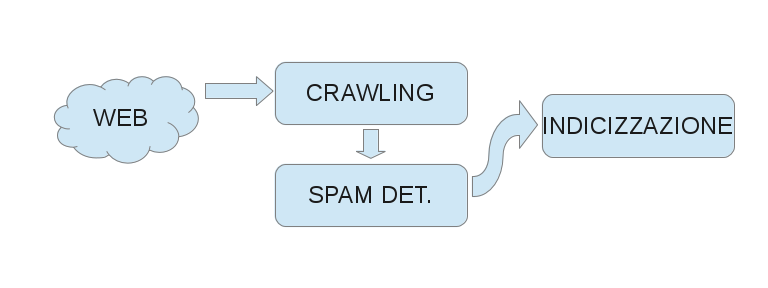
\includegraphics[width=10cm]{immagini/fasiSpam1}
  \end{center}
\end{frame}
\begin{frame}
    \frametitle{Spam Detection Online}
    Il rilevamento dello spam viene eseguito durante la fasi di crawling.
  \begin{center}
   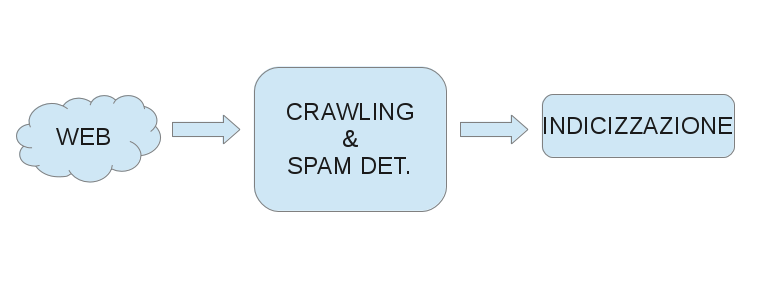
\includegraphics[width=10cm]{immagini/fasiSpam2}
  \end{center}
\end{frame}
\begin{frame}
    \frametitle{Tecniche di spam detection}
    \begin{block}<2->{Classificazione}
    \begin{itemize}
    \item<3->Tecniche basate sul contenuto;	
    \item<4->Tecniche basate sul grafo del web;
    \item<5->Tecniche basate su segnali eterogenei.
    \end{itemize}
    \end{block}
\end{frame}
\section{Tecniche basate sul contenuto}
\begin{frame}
    \frametitle{Tecniche basate sul contenuto - 1}
    Un metodo per identificare lo spam basandosi sul contenuto di una pagina web è  quello di analizzare alcune feature delle pagine spam e confrontarle con le medesime feature delle pagine non spam al fine di ottenere dei valori con cui stimare la natura della pagina web.
    \begin{block}<2->{Esempi di feature}
    \begin{itemize}
    \item Numero di parole all'interno della pagina (Keyword Stuffing);
    \item Numero di parole all'interno dei titoli delle pagine;
    \item Lunghezza media delle parole all'interno delle pagine;
    \item Lunghezza testo all'interno del tag \(<a>\);
    \item Frazione di contenuto visibile;
    \end{itemize}
    \end{block}
\end{frame}
\begin{frame}
    \frametitle{Feature: Numero di parole nel body}
  \begin{center}
  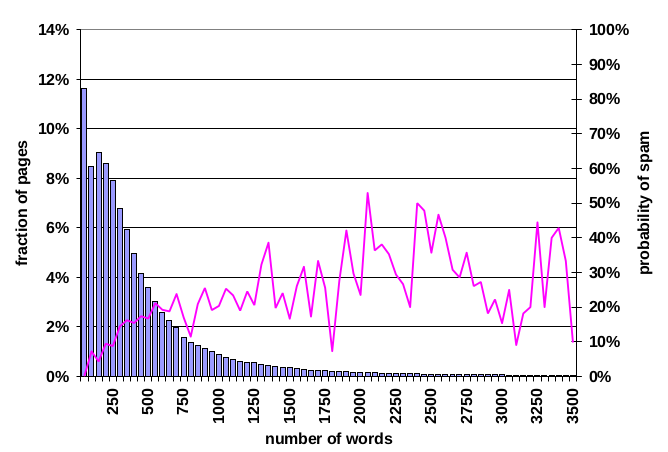
\includegraphics[width=8cm]{immagini/contenuto/fetterly3}
  \end{center}
\end{frame}
\begin{frame}
 \frametitle{Feature: Numero di parole nel titolo}
  \begin{center}
  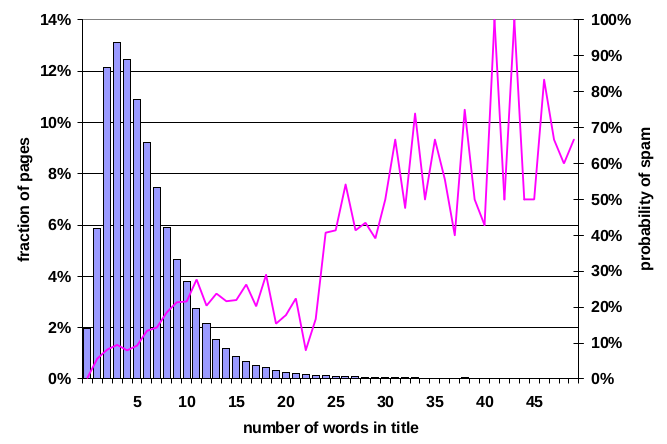
\includegraphics[width=8cm]{immagini/contenuto/fetterly4}
  \end{center}
\end{frame}
\begin{frame}
    \frametitle{Tecniche basate sul contenuto - 2}
    \begin{itemize}
     \item Viene utilizzata la \textit{Kullback-Leibler Divergence} (KLD) per misurare la divergenze tra le distribuzioni di probabilità dei termini	di pagine web, applicandola a unità di testo della pagina di partenza e di quella linkata
     \item La Kullback-Leibler (KL) è una misura  asimmetrica della divergenza che misura quanto male una distribuzione di probabilità \(M_q\) riesce a modellare \(M_d\)
     \begin{equation}
KLD(T_1||T_2) = \sum_{t \in T_1} P_{T_1}(t) \log \frac{P_{T_1}(t)}{P_{T_2}(t)}
\label{eqn:kld}
     \end{equation}
\end{itemize}
\end{frame}
\begin{frame}
  \frametitle{KLD: Tipo di sorgenti}
  \begin{block}<2->{Pagina di Partenza}
  \begin{itemize}
      \item testo delle ancore  
   \item testo intorno alle ancore
   \item termini nell'URL
  \end{itemize}
  \end{block}
  \begin{block}<3->{Pagina di Arrivo}
  \begin{itemize}
   \item titolo della pagina  
   \item contenuto della pagina
   \item meta tag
  \end{itemize}
  \end{block}
\end{frame}
\begin{frame}
  \frametitle{KLD: Uso delle sorgenti}
  \begin{block}{Combinazione}
  \begin{itemize}
      \item testo delle ancore - contenuto  
      \item testo vicino alle ancore - contenuto
      \item termini nell’URL - contenuto
      \item testo delle ancore - titolo
      \item testo intorno alle ancore - titolo
      \item termini nell’URL - titolo
      \item titolo - contenuto
      \item metatag
  \end{itemize}
  \end{block}
\end{frame}
\begin{frame}
  \frametitle{KLD: Uso delle sorgenti}
  \begin{block}{Combinazione}
  \begin{itemize}
      \item testo delle ancore - contenuto  
      \item testo vicino alle ancore - contenuto
      \item termini nell’URL - contenuto
      \item testo delle ancore - titolo
      \item testo intorno alle ancore - titolo
      \item termini nell’URL - titolo
      \item titolo - contenuto
      \item metatag
  \end{itemize}
  \end{block}
\end{frame}
\begin{frame}
  \frametitle{Tecniche basate sul grafo}
  \begin{block}{Tecniche base}
  \begin{itemize}
  \item TrustRank
  \item Anti-trust Rank
  \item Spam mass
  \end{itemize}
  \end{block}
  \begin{block}<2->{}
  Utilizzano una versione personalizzata di PageRank:
  \begin{equation}
   \alpha G + (1-\alpha)1v^t
   \label{eqn:pagerank}
  \end{equation}
  \end{block}
  \end{frame}
\begin{frame}
  \frametitle{TrustRank}
  TrustRank tenta di assegnare un valore di rank maggiore alle pagine non spam rispetto alle pagine spam partendo da un insieme di pagine non spam.
  \begin{block}<2->{Assunzione}
  \begin{itemize}
   \item Per determinare le pagine non spam, viene fatta un’assunzione empirica chiamata isolazione approssimata dell’insieme delle pagine buone, la quale afferma che le pagine non spam raramente punteranno a delle pagine spam.
   \item Gli sviluppatori di pagine web non spam non hanno interesse nel linkare pagine spam (a meno che tramite l’uso di tecniche come l’honeypot vengano “ingannati”).
  \end{itemize}
  \end{block}
\end{frame}
\begin{frame}
  \frametitle{TrustRank}
  \begin{itemize}
   \item   TrustRank quindi è una versione personalizzata di PageRank dove il vettore di preferenza \(v\) non rappresenta una distribuzione uniforme su tutte le pagine del grafo \(G\) ma una distribzione personalizzata dalle pagine del seedset di partenza.
$$
   \alpha G + (1-\alpha)1v^t
$$
\item I campi del vettore \(v\) avranno valore 1 se corrisponderanno al nodo del seedset altrimenti 0.
  \end{itemize}
\end{frame}
\begin{frame}
  \frametitle{Anti-trust Rank}
  \begin{itemize}
   \item Partendo dalla stessa intuizione dell'isolamento approsimato 
   \item Anti-trust Rank utilizza un seed set iniziale composto da pagine spam
   \item Quindi una pagina spam (conosciuta) è linkata da un'altra pagina spam in quanto una pagina non spam non ne avrebbe il motivo 
   \item Come per TrustRank, Anti-trust Rank viene calolato usando Pagerank personalizzato sul grafo trasposto (visto che adesso si prendono in consierazioni i link in entrata)
   \item Anti-trust Rank assegna un rank maggiore alle pagine spam
  \end{itemize}
\end{frame}
\begin{frame}
  \frametitle{Spam mass}
  \begin{itemize}
   \item Per riconoscere una spam farm si parte dal presupposto che i nodi della spam farm hanno dei link uscenti verso delle pagine target \(t\) per aumentarne il rank
   \item Spam mass è una misura che valuta l'impatto dello spam sul rank di una pagina
   \item Vengono assegnati due valori: PageRank e Spam mass
  \end{itemize}
\end{frame}
\begin{frame}
  \frametitle{Determinazione della spam farm}
  Partendo da un insieme \(\tilde{(V)}^+\) composto da pagine non spam conosiute
   \begin{block}<2->{Si calcolano due misure}
   \begin{itemize}
    \item Spam mass assoluta: \(\tilde{M}_x=p_x-p'_x\)
     \item Spam mass relativa:  \(\tilde{m}_x=(p_x-p'_x)/p_x=1-p'_x/px\)
   \end{itemize}
   dove \(p\) è il \textit{pagerank} dei nodi basato su una distribuzione uniforme mentre \(p'\) è \textit{pagerank} basato sull'insieme \(\tilde{(V)}^+\).
   
   Viene usato un valore di soglia per determinare se una pagina è parte di una spam farm.
   \end{block}
\end{frame}
\begin{frame}
  \frametitle{Tecniche eterogenee}
  Partendo da un insieme \(\tilde{(V)}^+\) composto da pagine non spam conosiute
   \begin{block}<2->{Si calcolano due misure}
   \begin{itemize}
    \item Spam mass assoluta: \(\tilde{M}_x=p_x-p'_x\)
     \item Spam mass relativa:  \(\tilde{m}_x=(p_x-p'_x)/p_x=1-p'_x/px\)
   \end{itemize}
   dove \(p\) è il \textit{pagerank} dei nodi basato su una distribuzione uniforme mentre \(p'\) è \textit{pagerank} basato sull'insieme \(\tilde{(V)}^+\).
   
   Viene usato un valore di soglia per determinare se una pagina è parte di una spam farm.
   \end{block}
\end{frame}

\end{document}
